\clearpage
\section{Thực nghiệm và đánh giá}
\subsection{Thiết lập thực nghiệm}
% Bộ 9 puzzle: 3x3, 4x4, 5x5; 5 lượt/puzzle; timeout 30 giây/lượt.
% Điền cấu hình CPU/RAM/OS/Python thực tế nếu xác minh được.
% Phân biệt thời gian giải tuần tự và thời gian kiểm tra uniqueness.
\subsection{Chỉ số đánh giá}
% Primary variables, auxiliary variables, CNF clauses, SAT calls,
% decisions, propagations, backtracks, deduction steps, runtime.
\subsection{Kết quả theo kích thước bàn cờ}
\begin{figure}[htbp]\centering
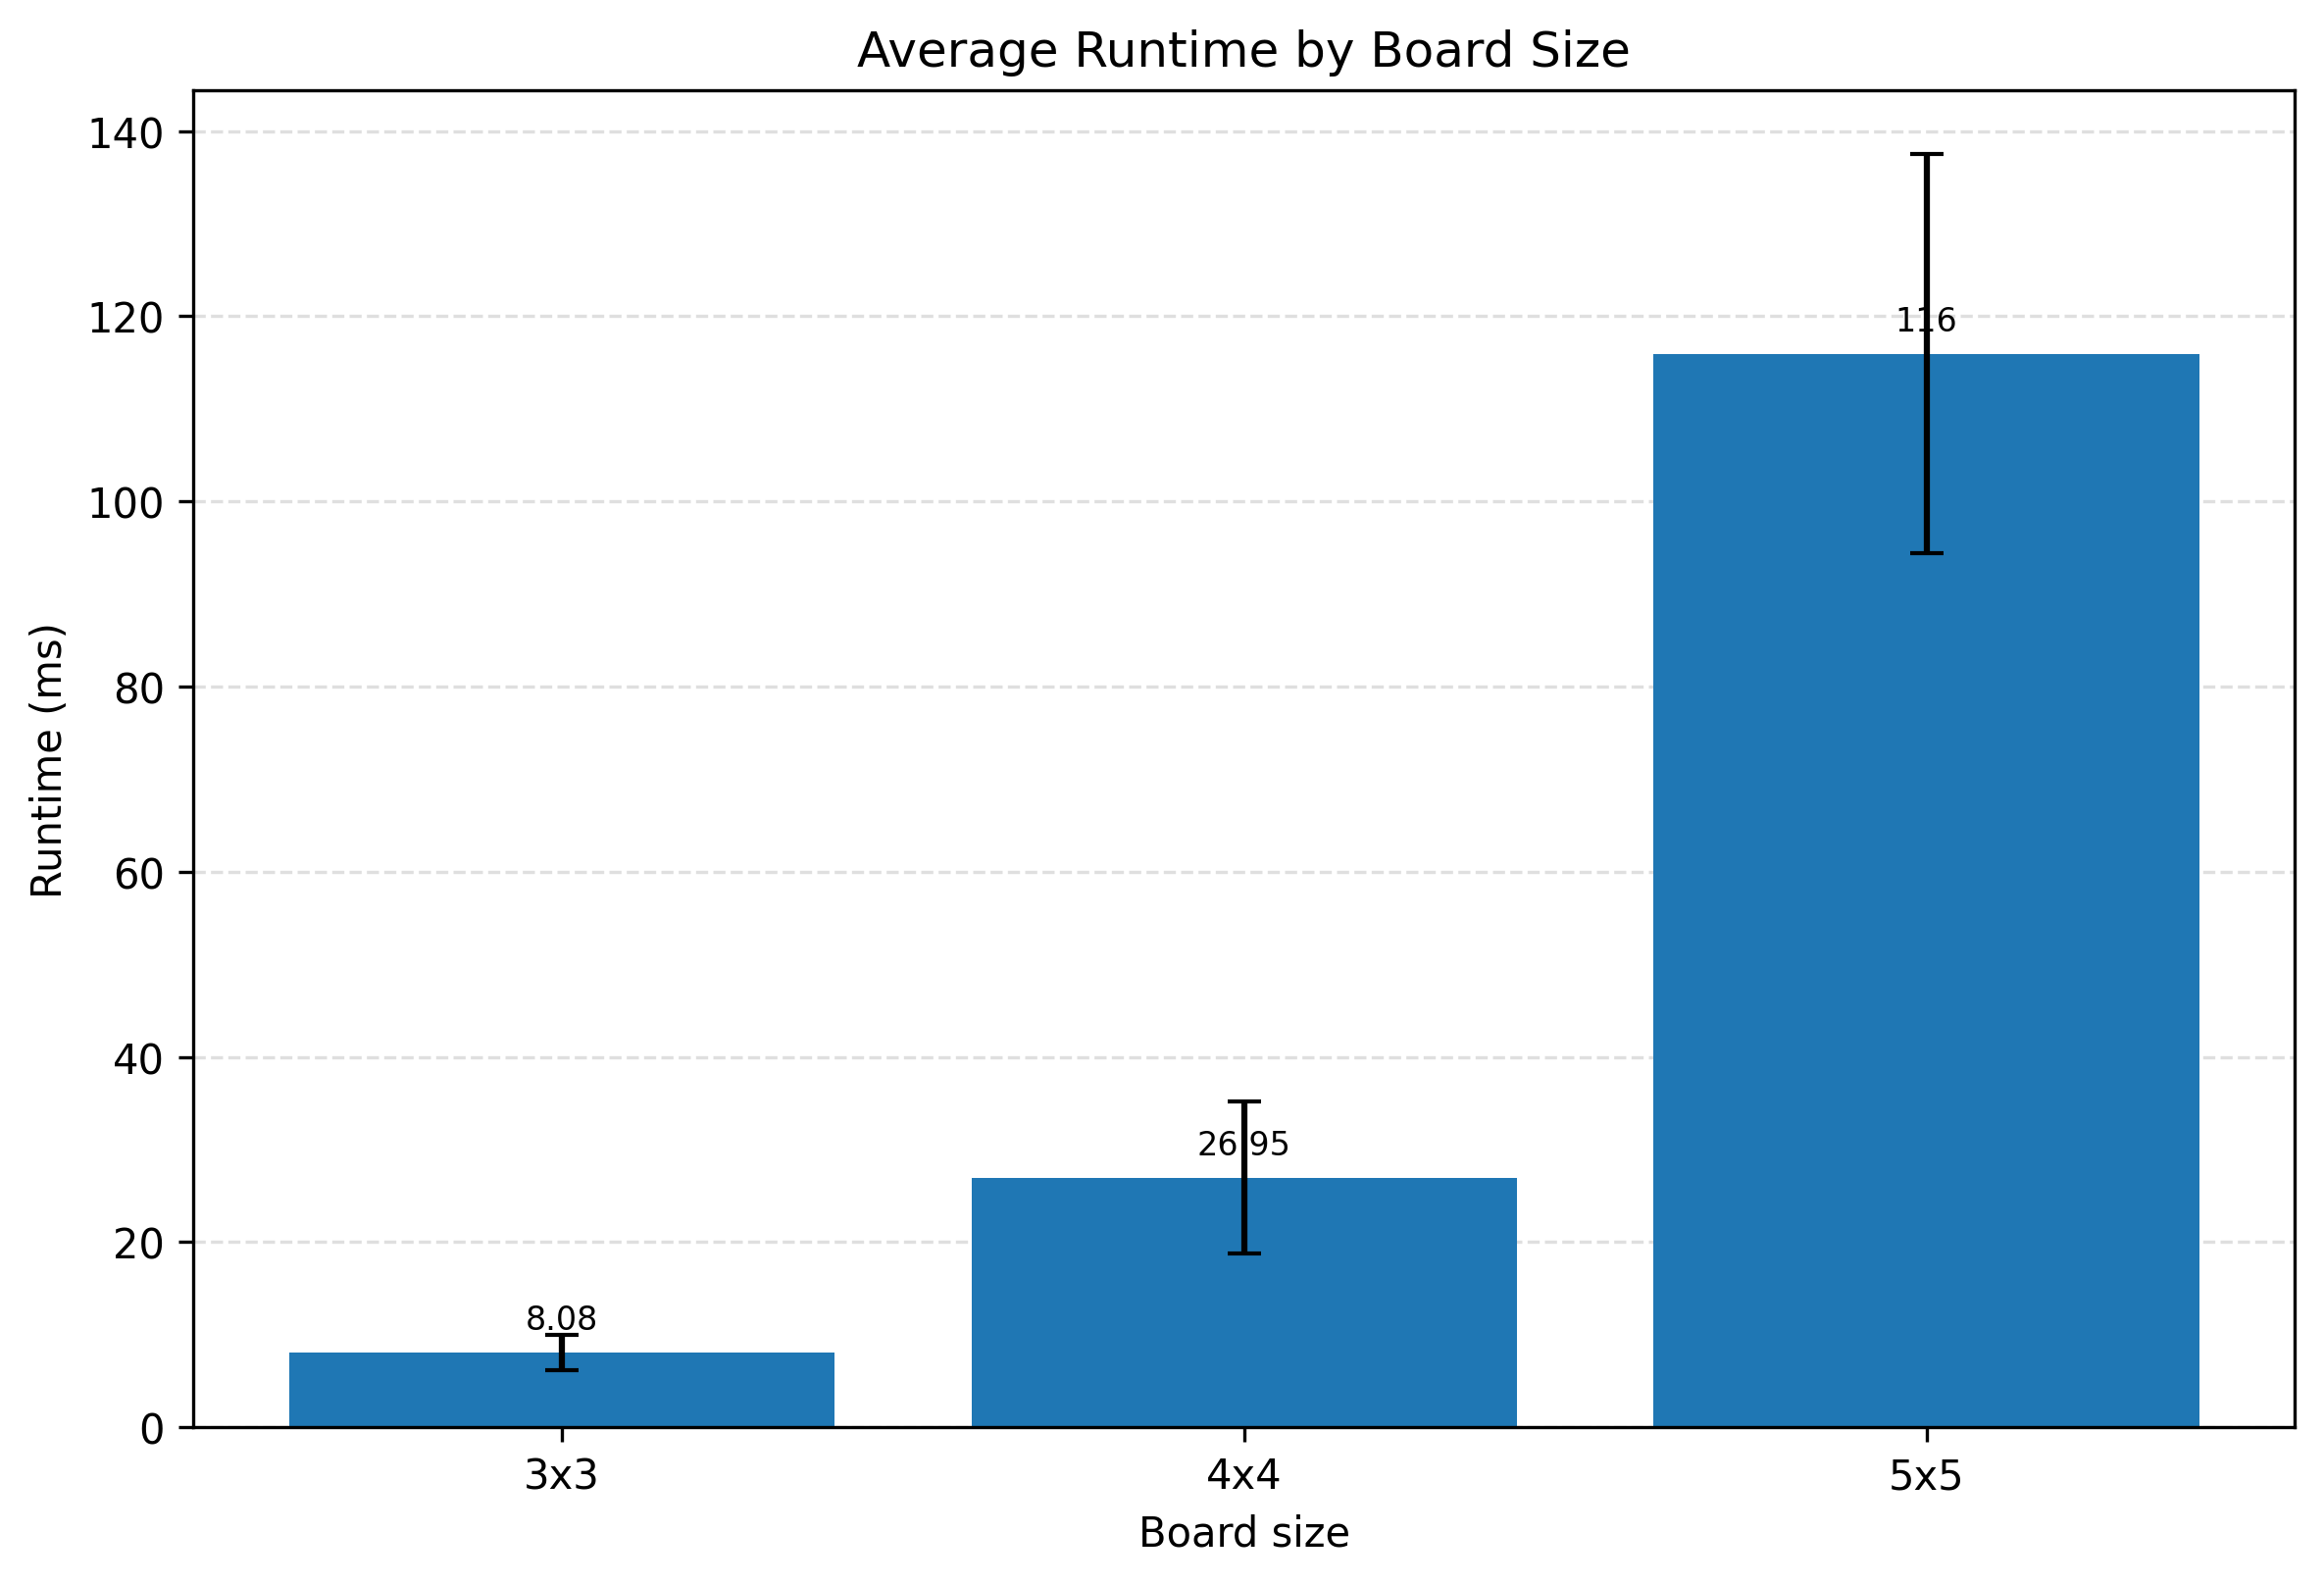
\includegraphics[width=0.88\linewidth]{runtime_by_size.png}
\caption{Runtime trung bình theo kích thước bàn cờ.}
\end{figure}
\begin{figure}[htbp]\centering
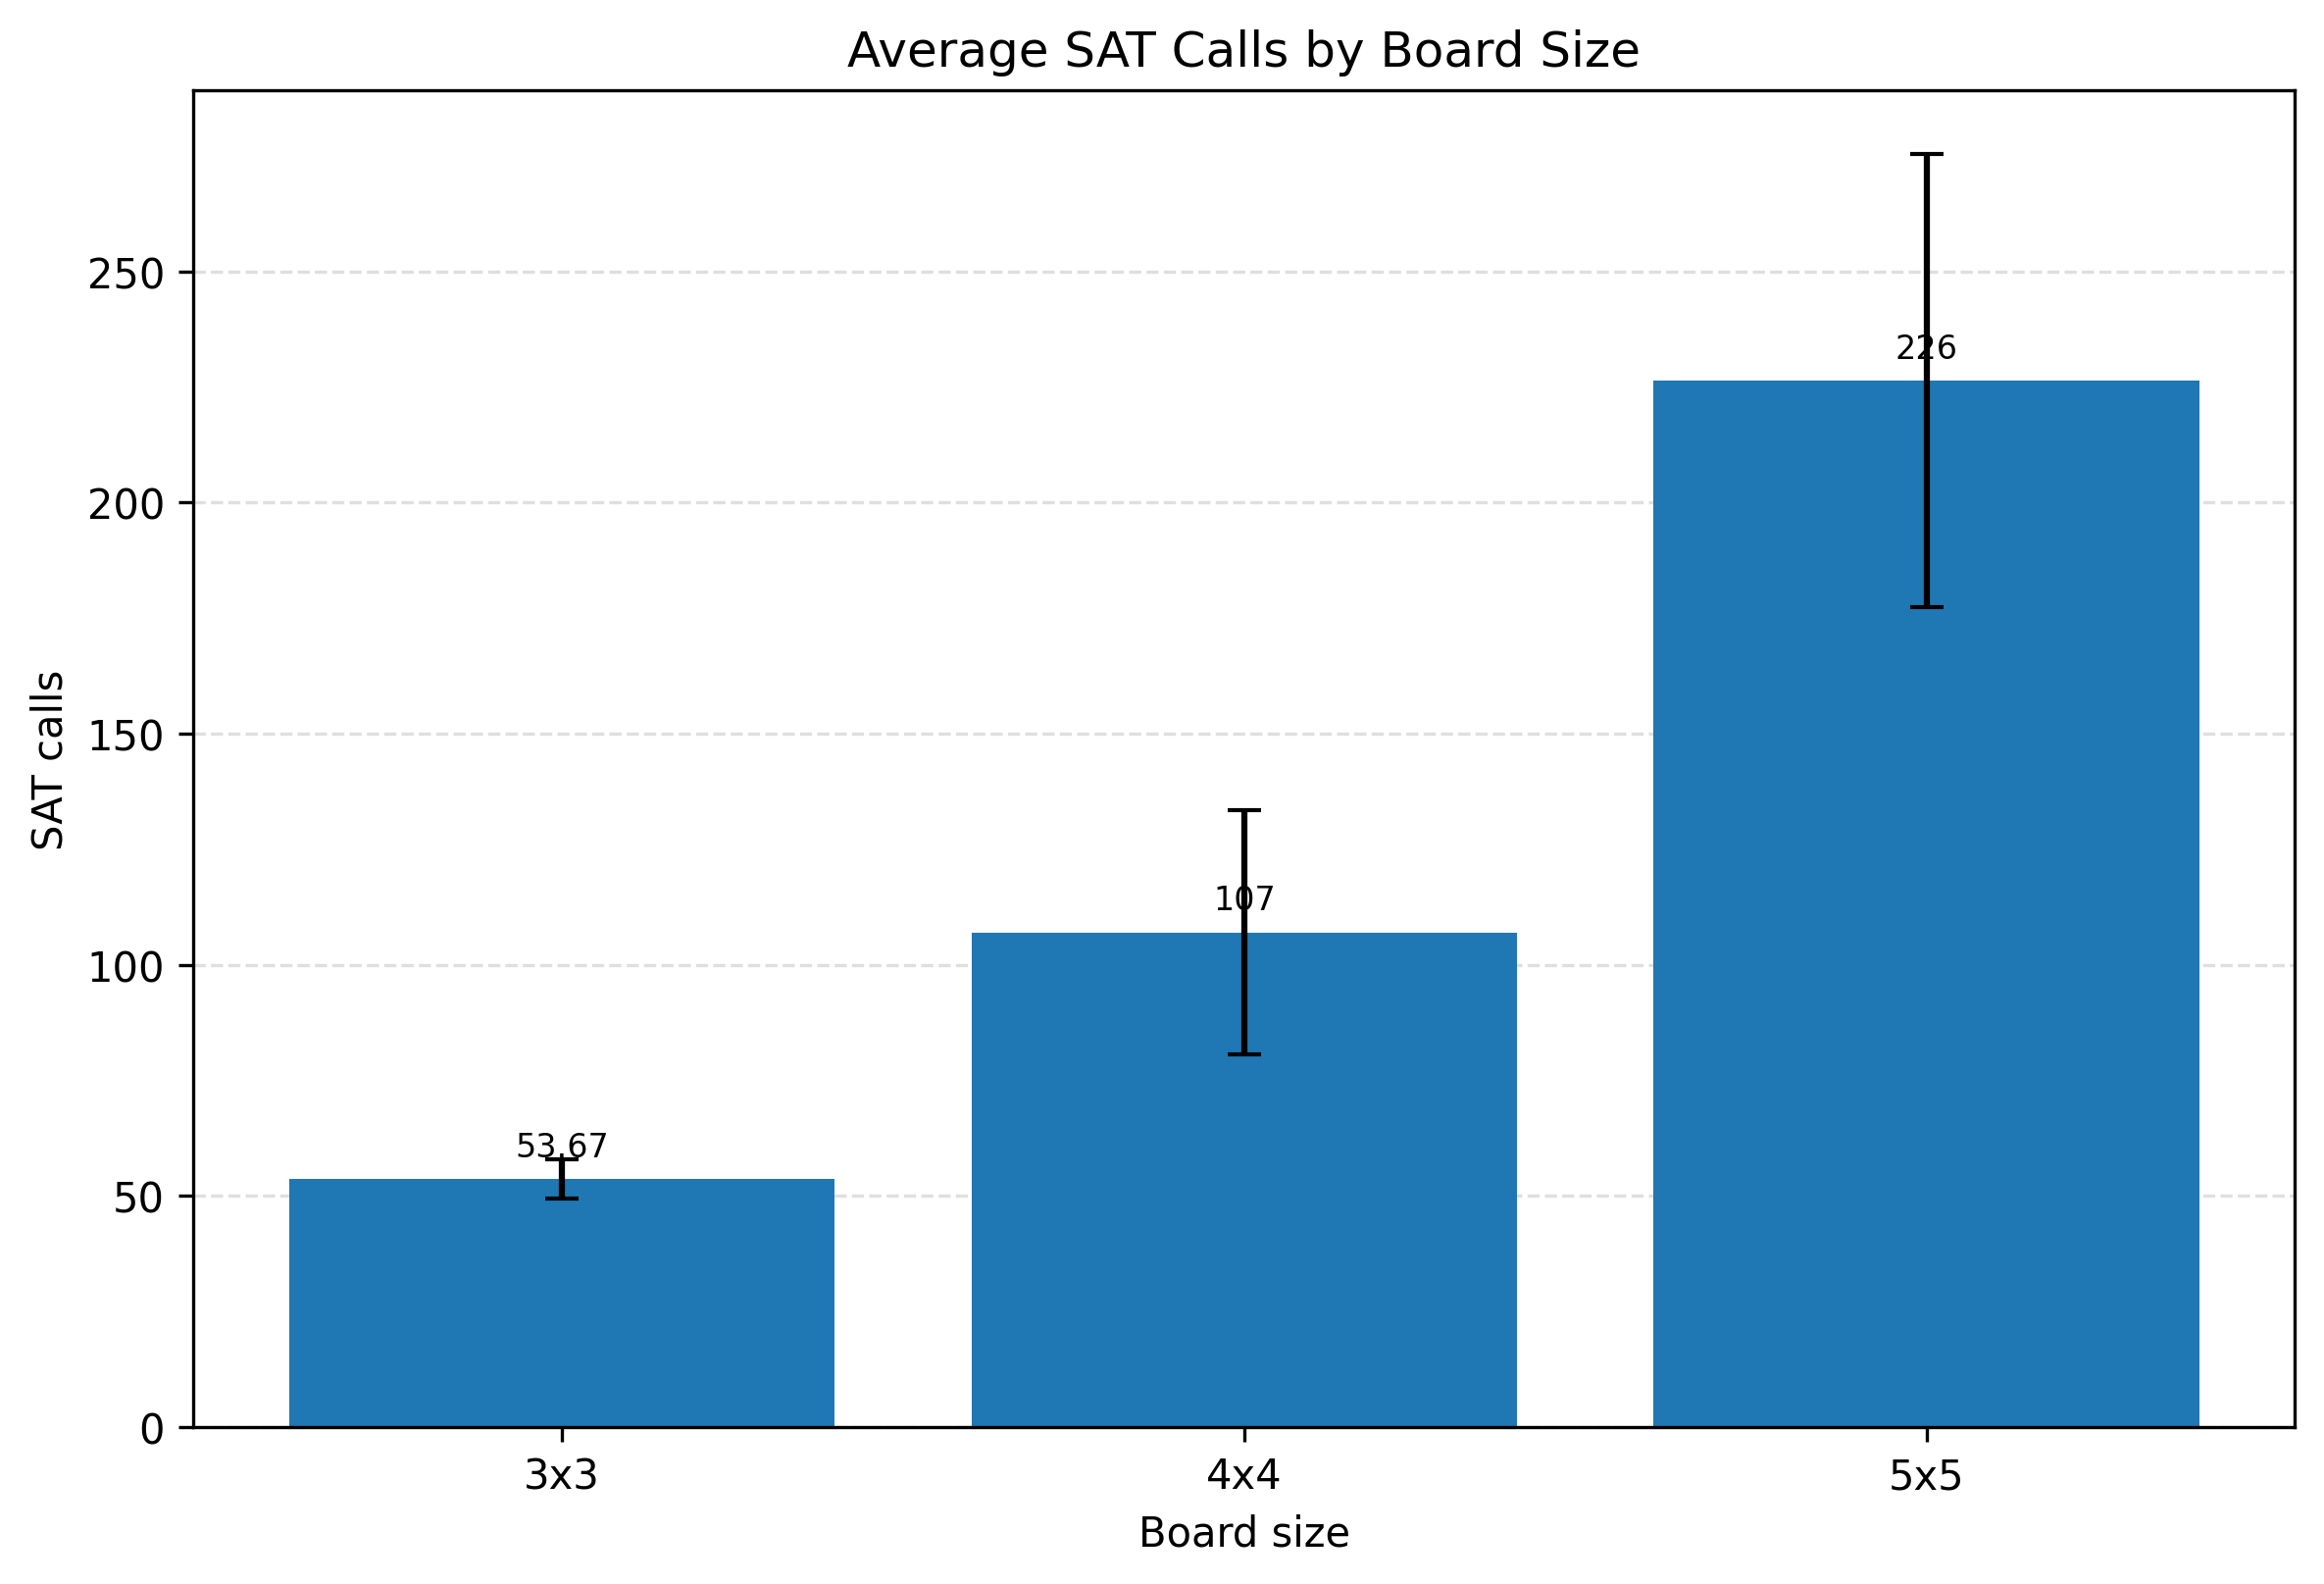
\includegraphics[width=0.88\linewidth]{sat_calls_by_size.png}
\caption{Số lần gọi SAT trung bình theo kích thước.}
\end{figure}
\begin{figure}[htbp]\centering
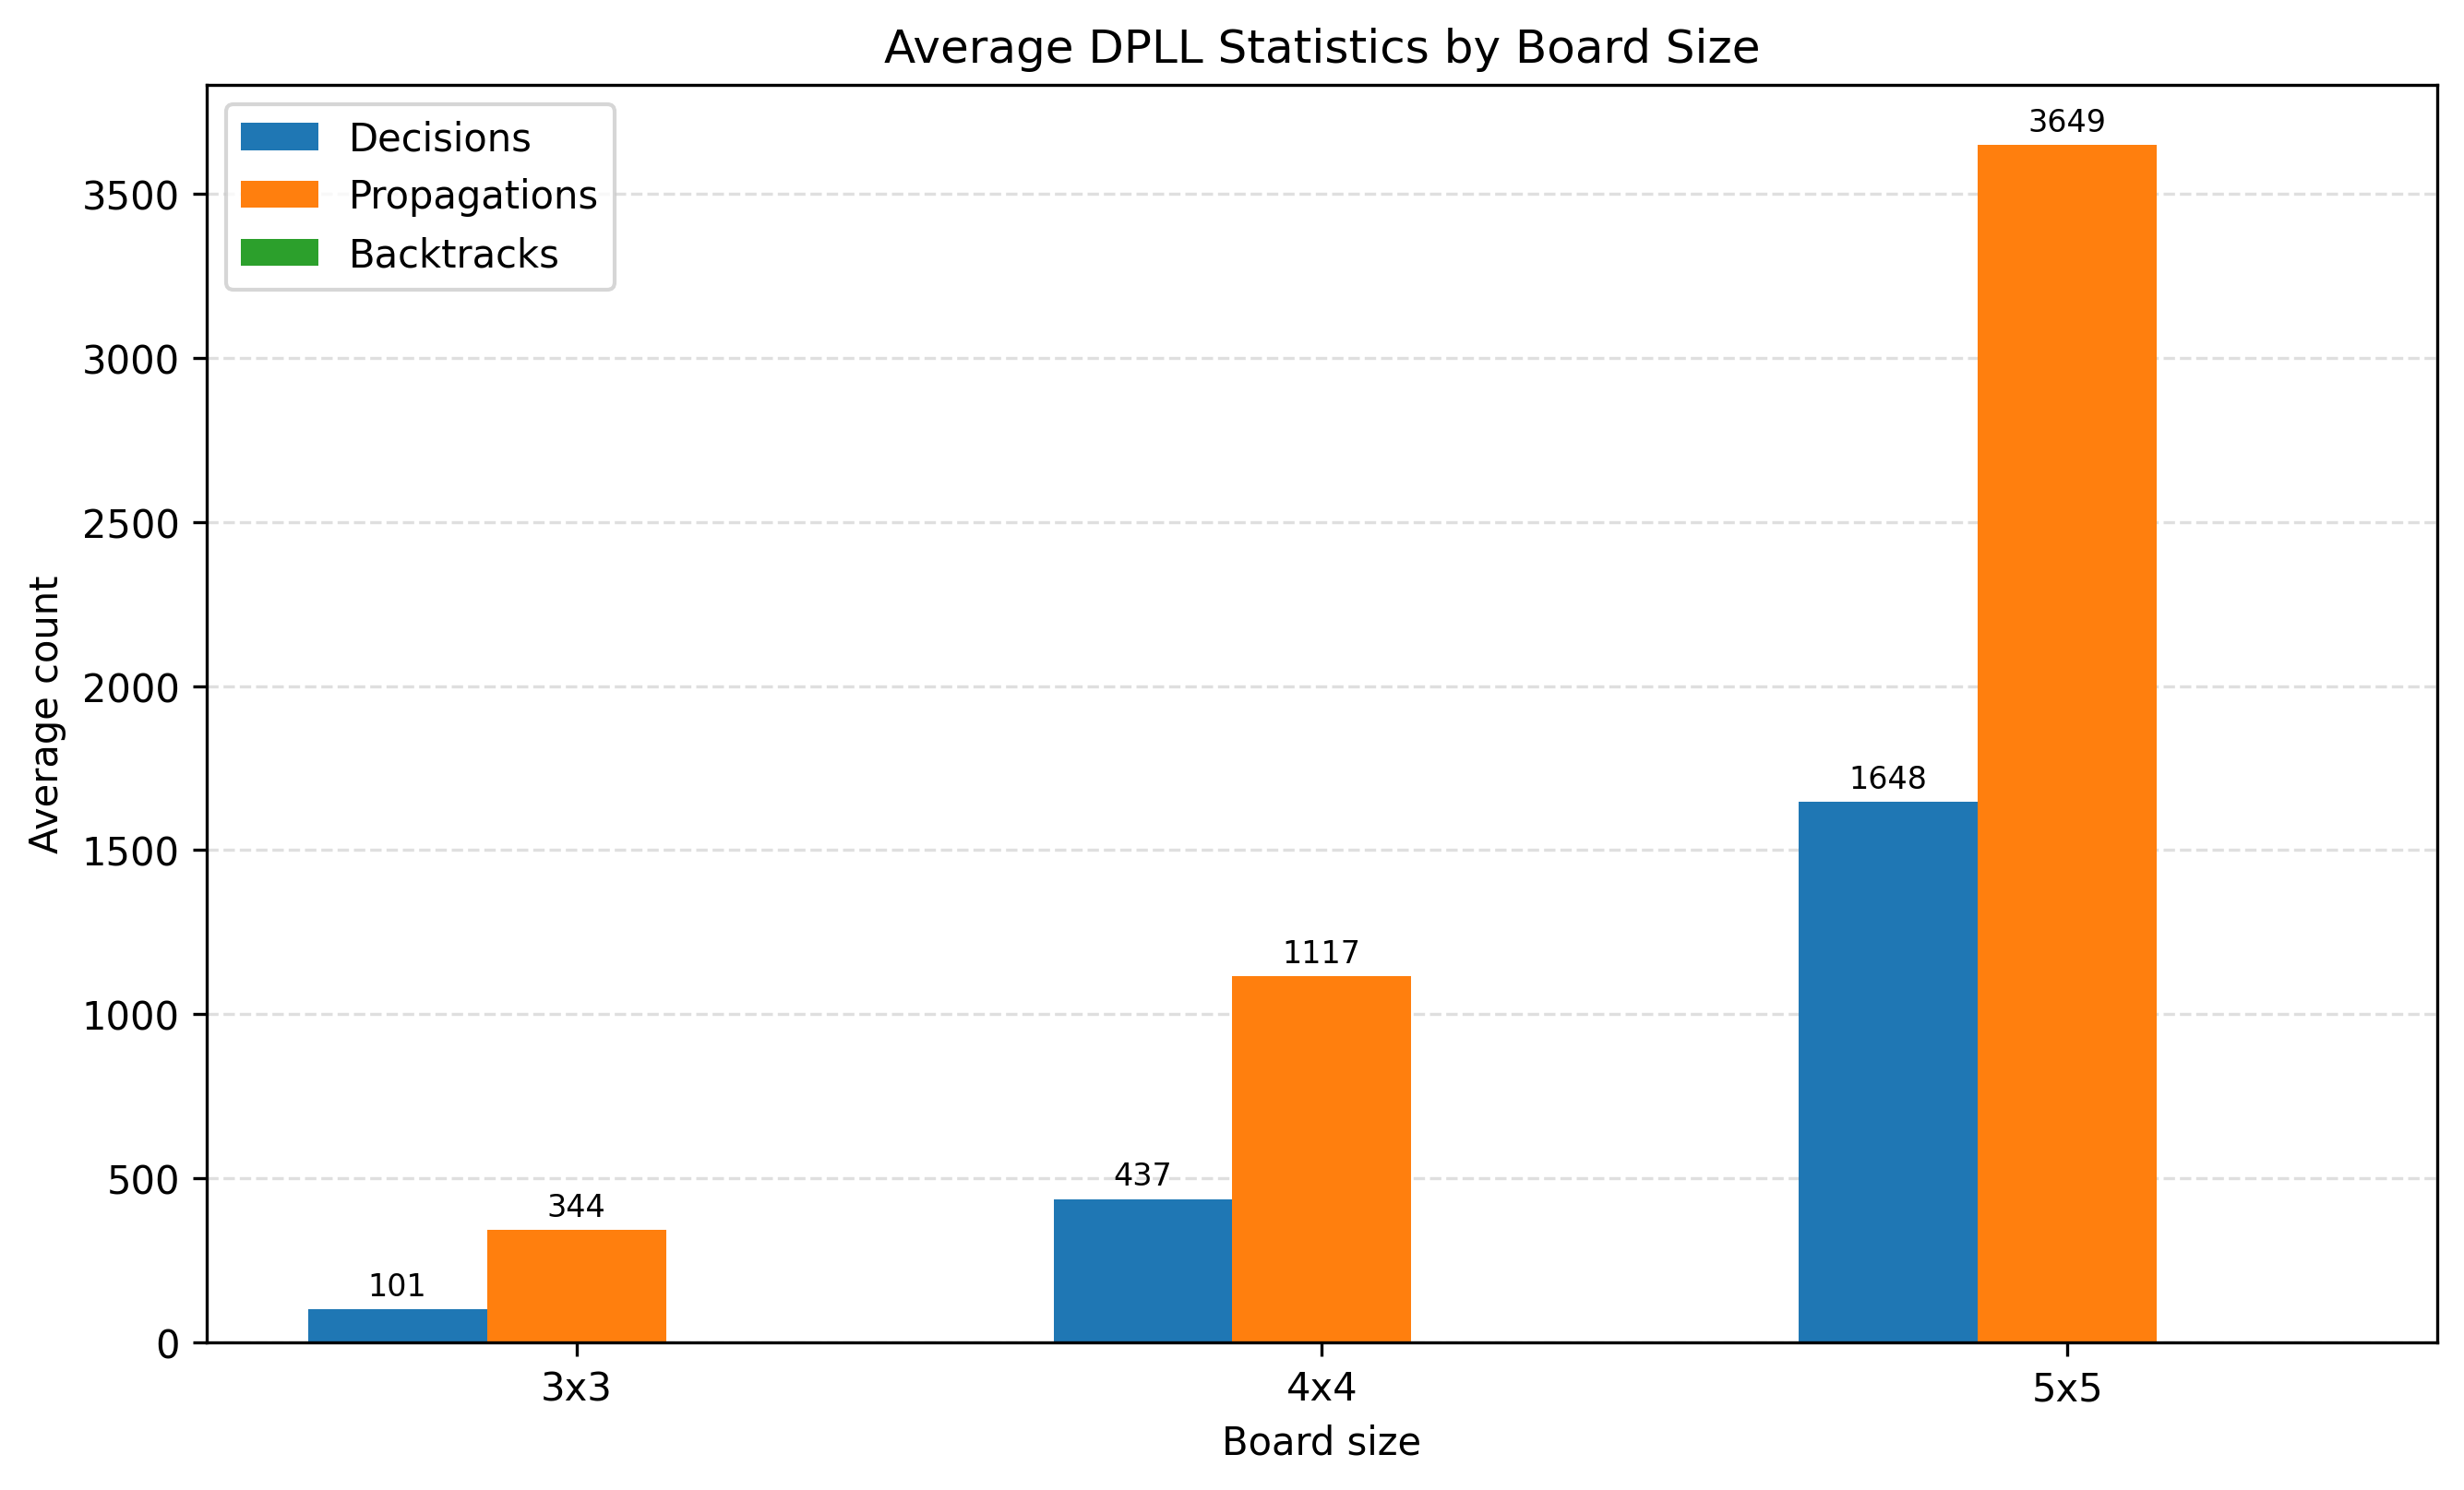
\includegraphics[width=0.88\linewidth]{dpll_statistics_by_size.png}
\caption{Các thống kê DPLL theo kích thước bàn cờ.}
\end{figure}
\subsection{Kết quả theo từng màn chơi}
\begin{figure}[htbp]\centering
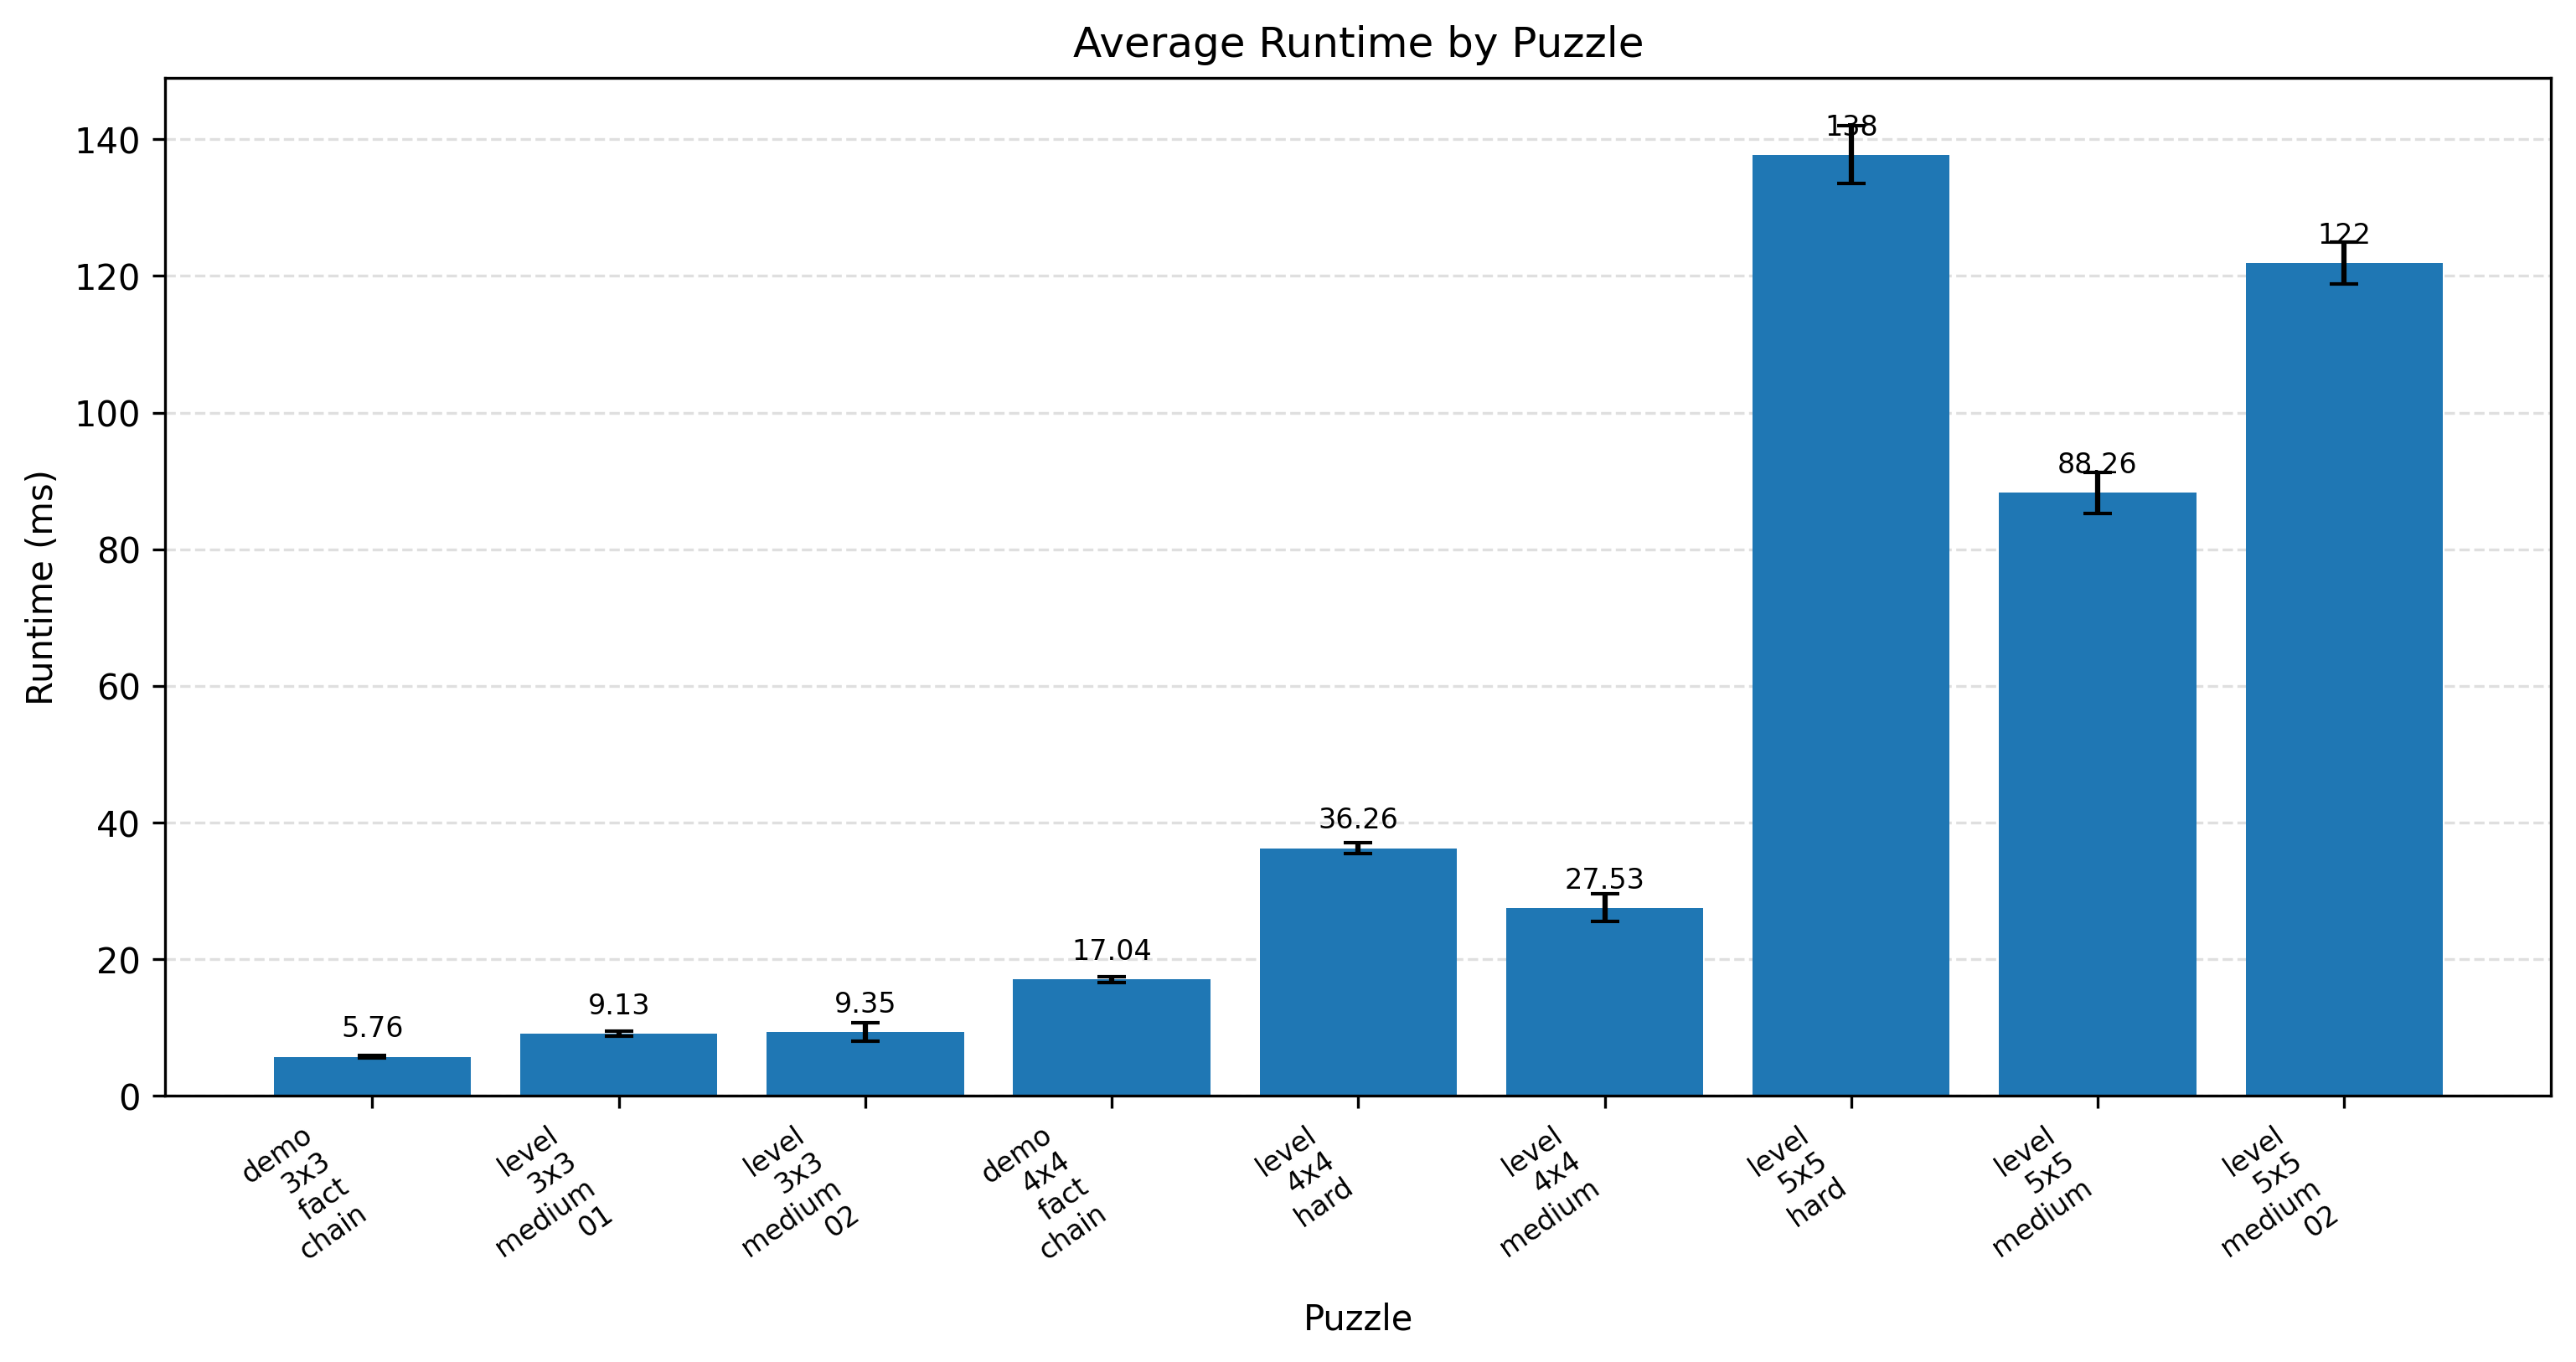
\includegraphics[width=\linewidth]{runtime_by_puzzle.png}
\caption{Runtime trung bình của từng puzzle.}
\end{figure}
\begin{figure}[htbp]\centering
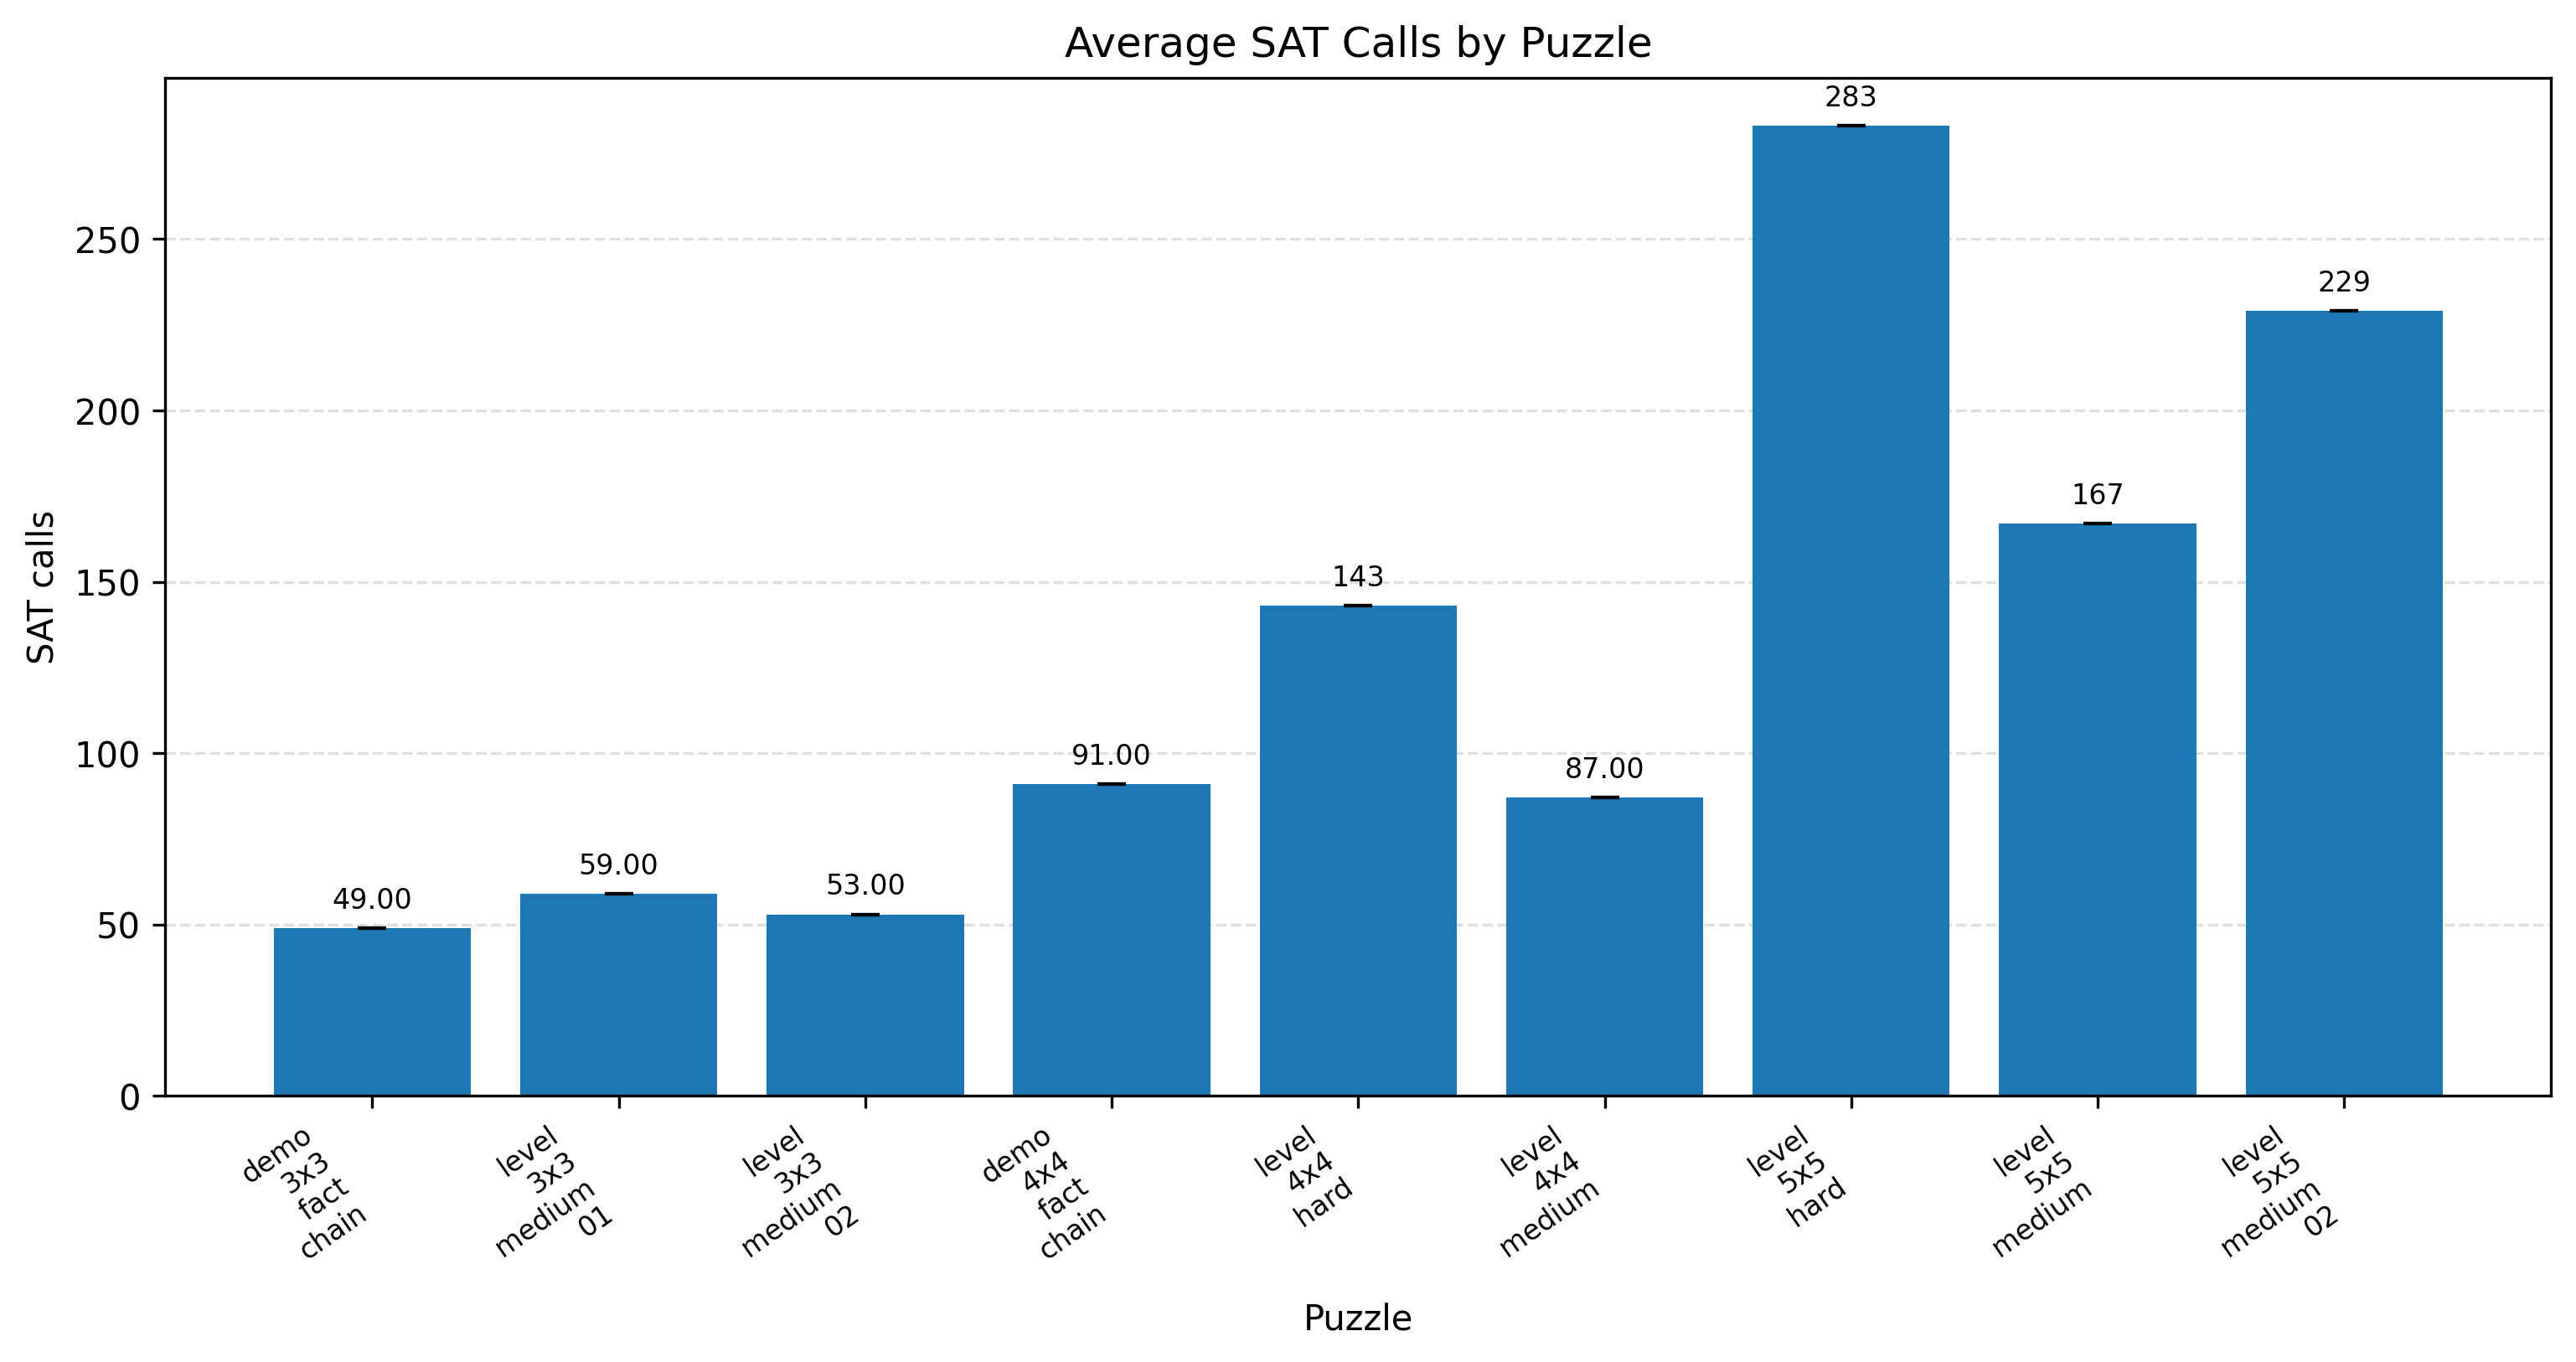
\includegraphics[width=\linewidth]{sat_calls_by_puzzle.png}
\caption{Số lần gọi SAT của từng puzzle.}
\end{figure}
\begin{figure}[htbp]\centering
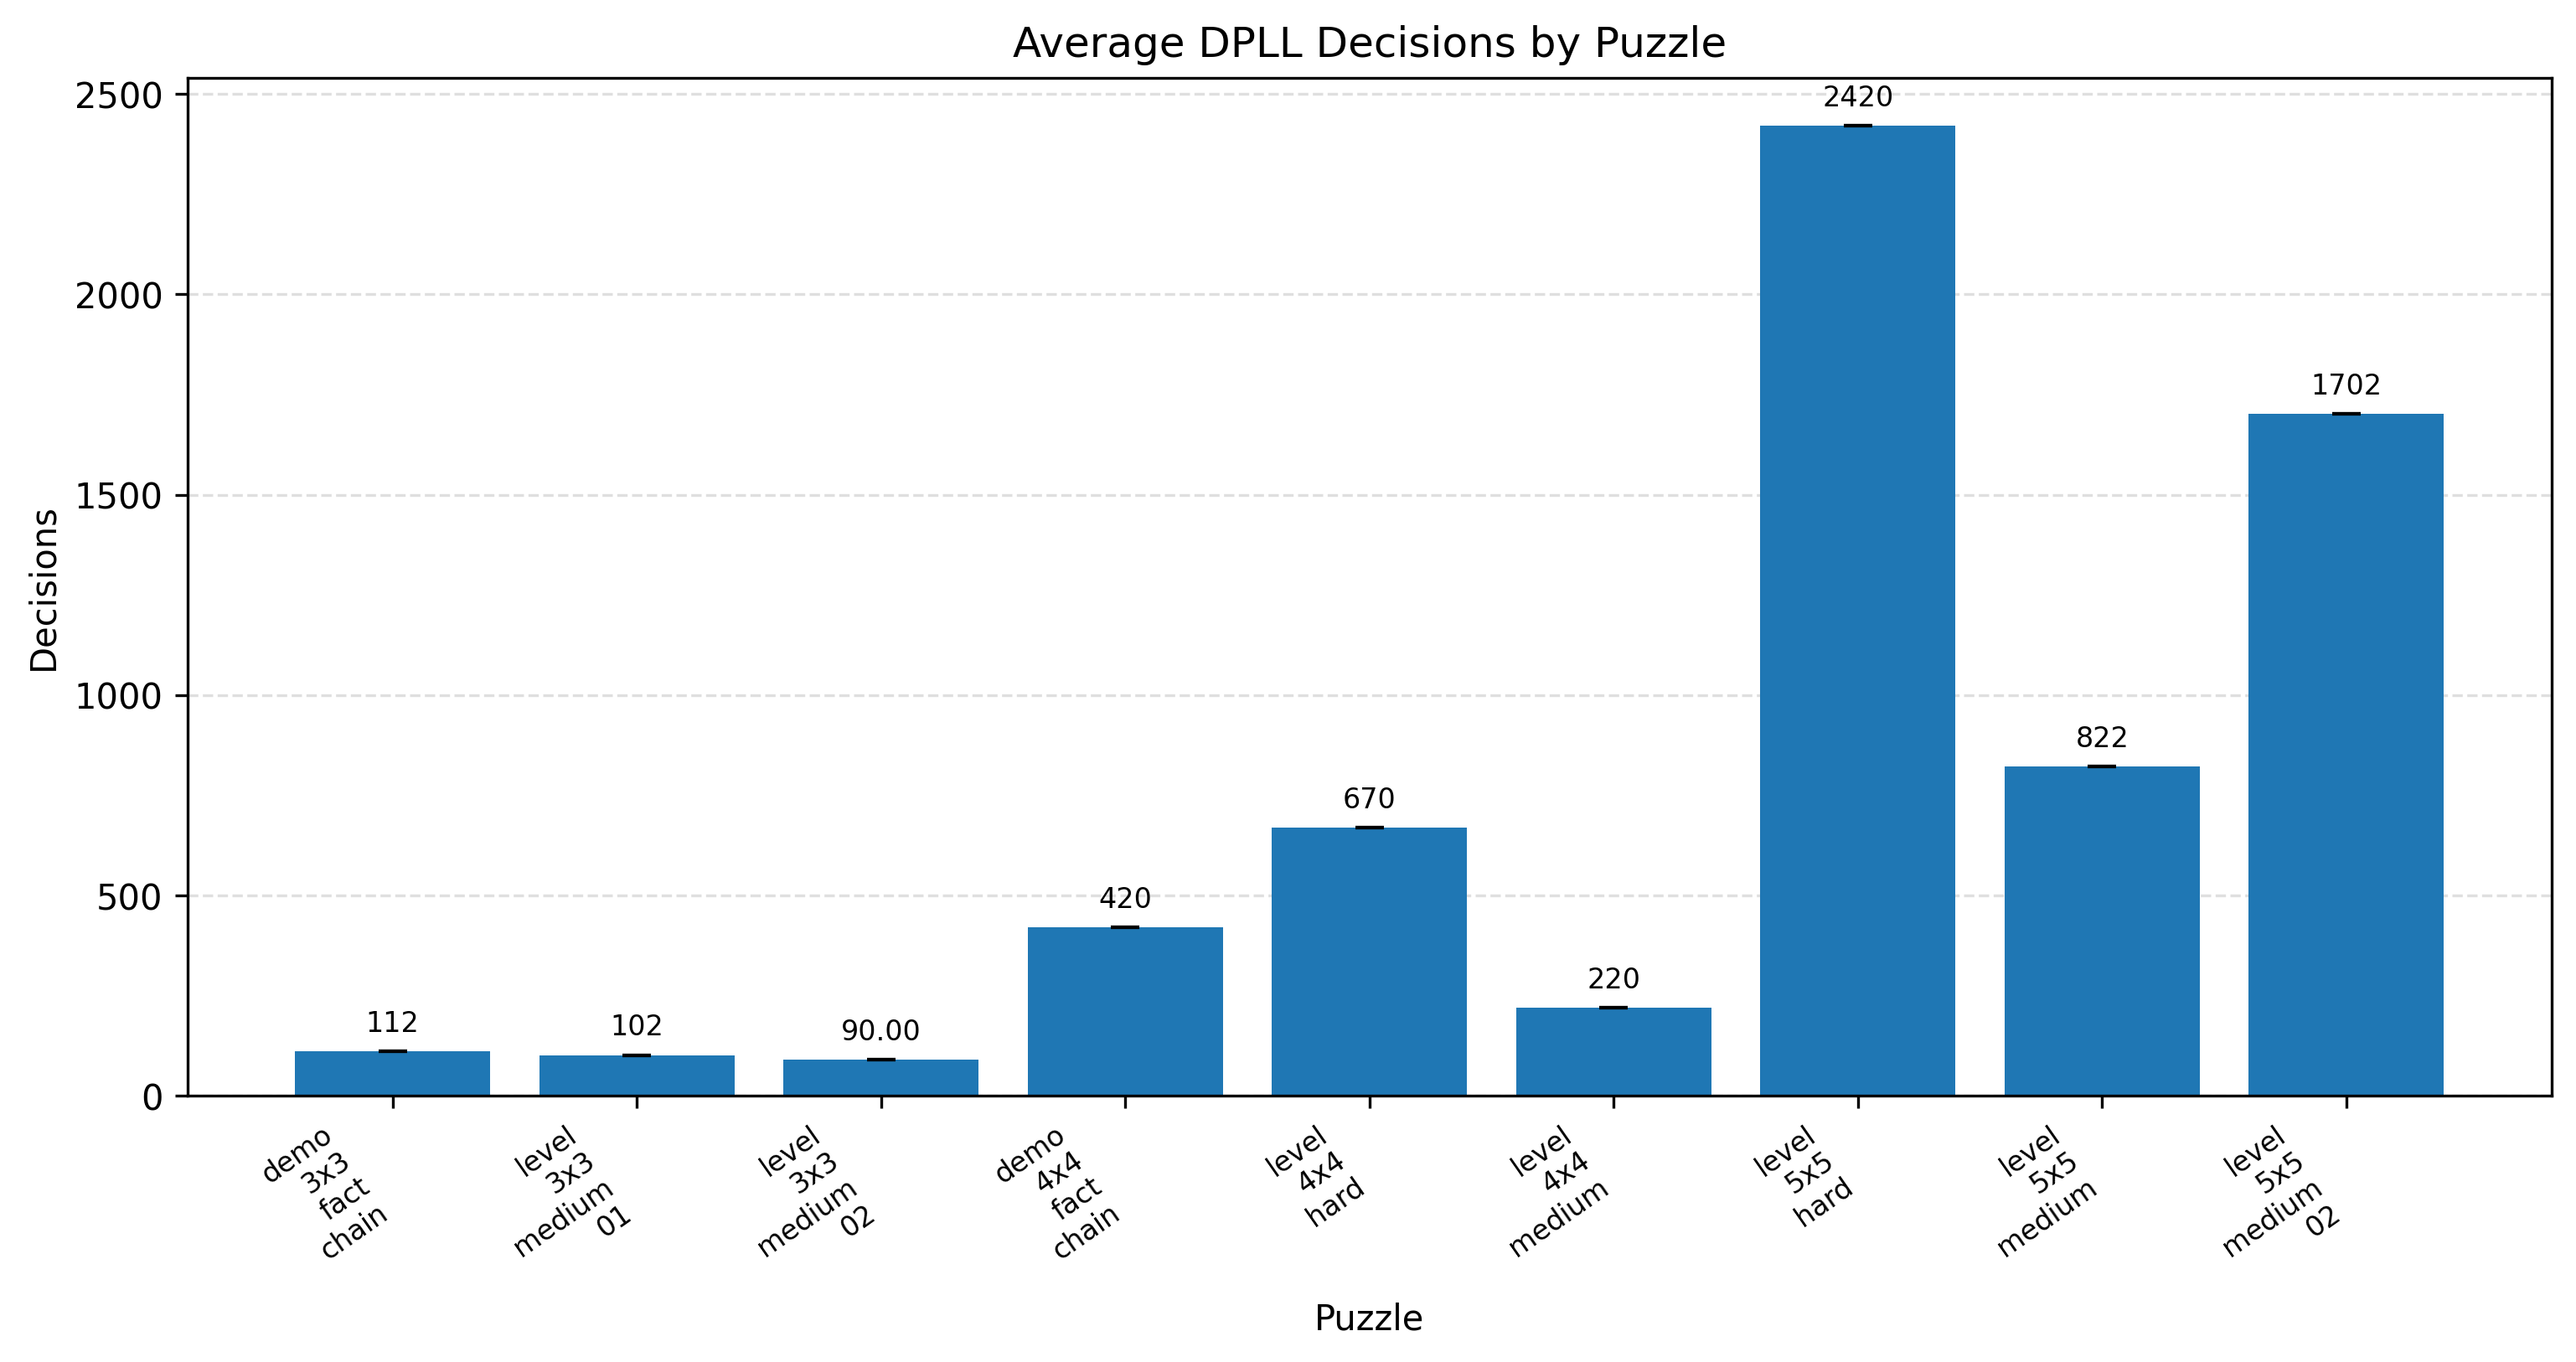
\includegraphics[width=\linewidth]{decisions_by_puzzle.png}
\caption{Số decisions của từng puzzle.}
\end{figure}
\begin{figure}[htbp]\centering
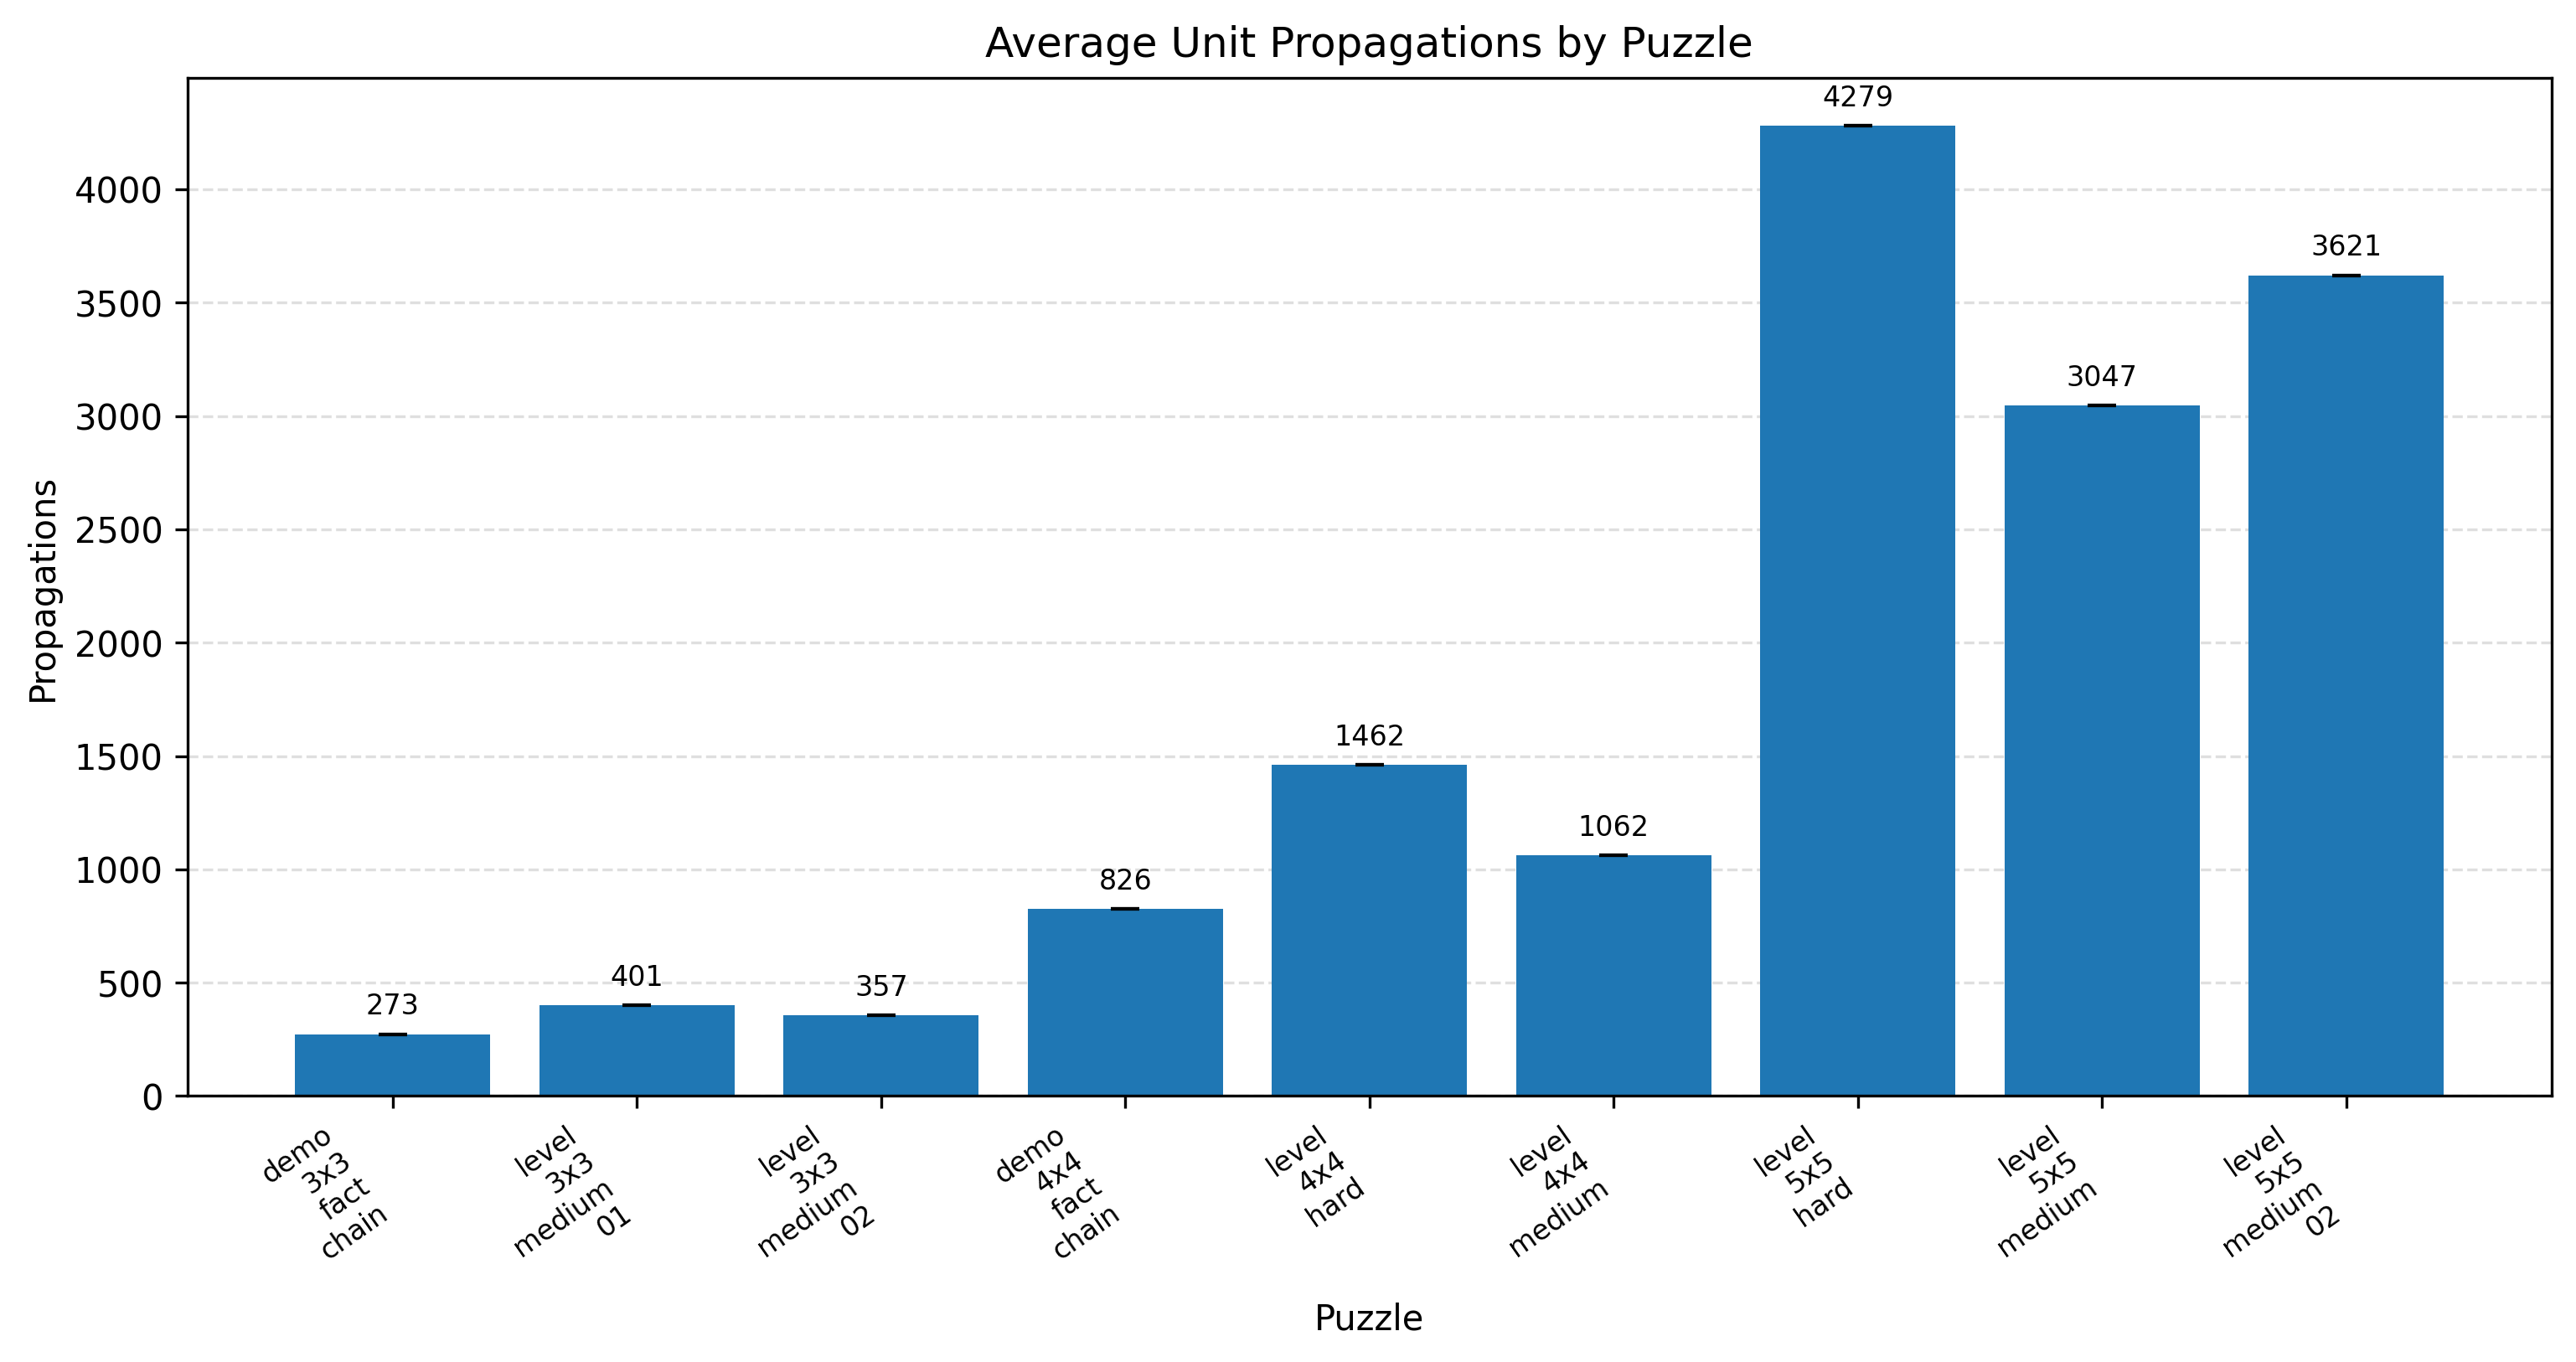
\includegraphics[width=\linewidth]{propagations_by_puzzle.png}
\caption{Số propagations của từng puzzle.}
\end{figure}
\begin{figure}[htbp]\centering
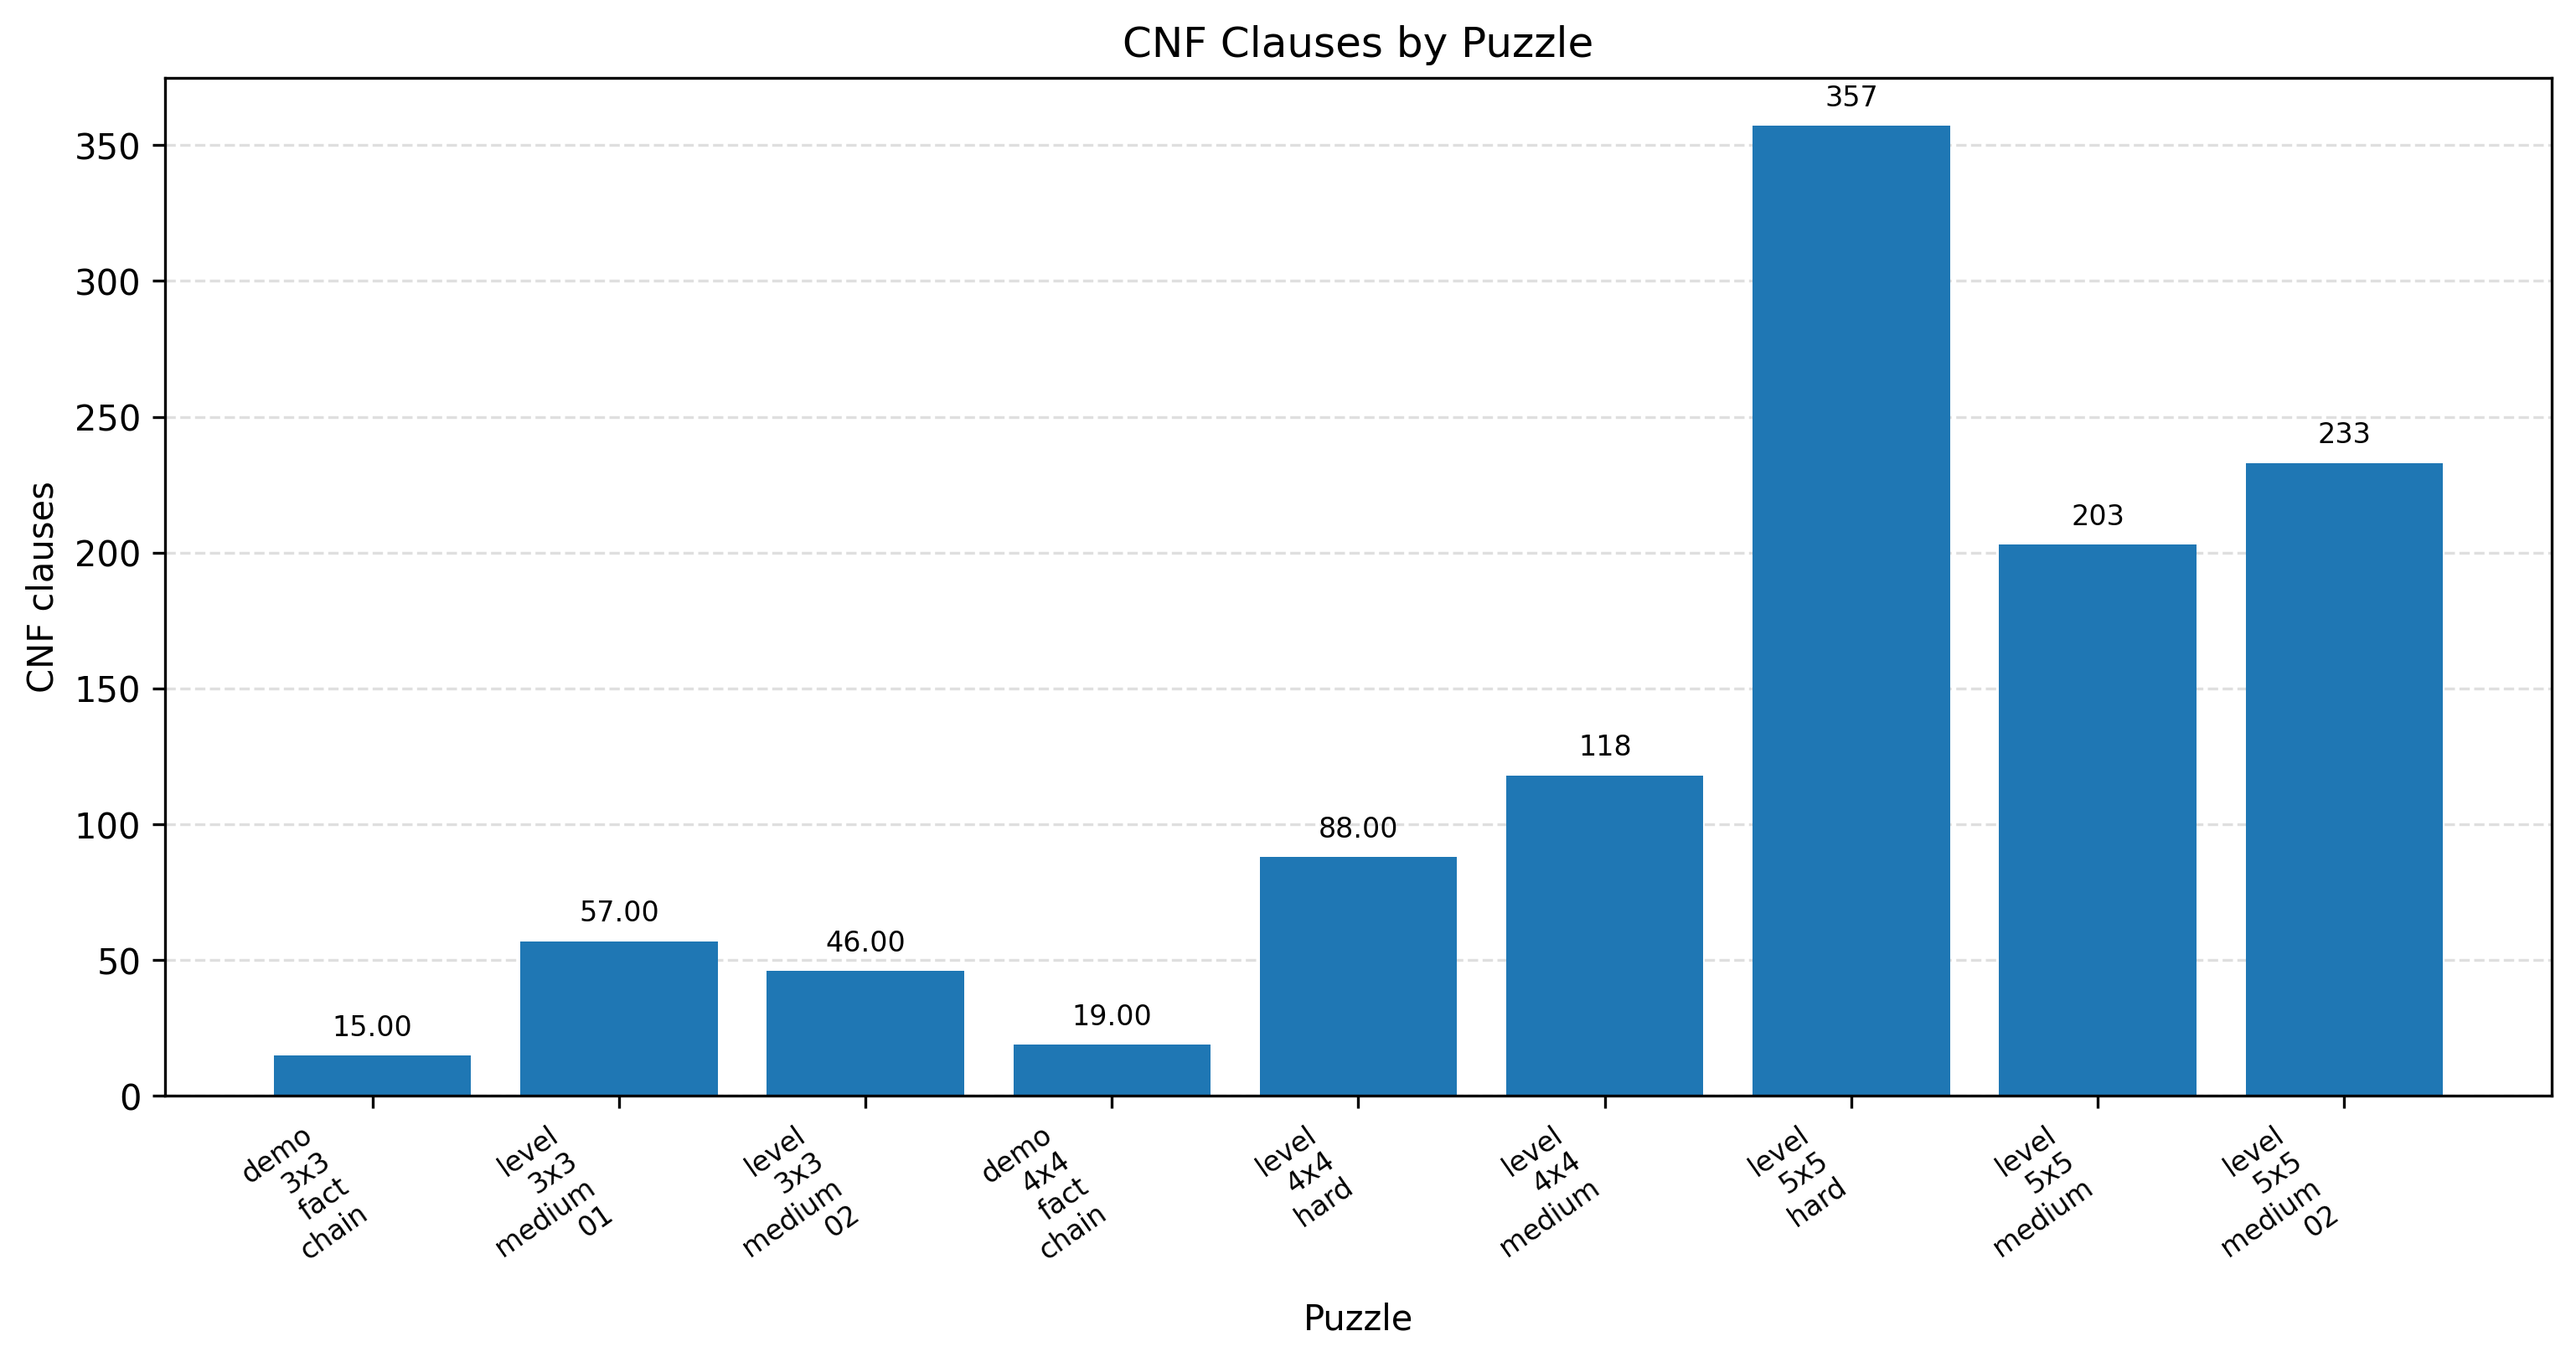
\includegraphics[width=\linewidth]{cnf_clauses_by_puzzle.png}
\caption{Số CNF clauses của từng puzzle.}
\end{figure}
\subsection{Phân tích kết quả}
% Phân tích số liệu từ experiment_size_summary.csv và experiment_summary.csv.
% Không suy rộng ngoài 9 puzzle/45 lượt chạy.
\subsection{Trường hợp đặc biệt và hạn chế}
% Báo cáo demo_4x4 MULTIPLE nhưng SOLVED(5/5) đúng thực tế hiện tại.
% Nêu rõ đây là tính duy nhất khác với khả năng giải tuần tự.
% Cập nhật lại nếu nhóm thay puzzle và chạy lại thí nghiệm.
